\documentclass[fleqn,10pt,lineno]{manuscript}
%%\usepackage{setspace}
%%\doublespacing
\usepackage{soul}
\usepackage[utf8]{inputenc}

\newcommand{\beginsupplement}{%
        \setcounter{table}{0}
        \renewcommand{\thetable}{S\arabic{table}}%
        \setcounter{figure}{0}
        \renewcommand{\thefigure}{S\arabic{figure}}%
     }

\title{A Structural and Functional Bioinformatics Study of QTY-designed Retinylidene Proteins}

\author[1]{Siqi Pan}
\author[2]{Shuguang Zhang}
\affil[1]{Shanghai World Foreign Language Academy, 400 Baihua Street, Shanghai 200233, China}
\affil[2]{Lab of Molecular Architecture, Media Lab, Massachusetts Institute of Technology, 77 Massachusetts Avenue, Cambridge, MA 02139, USA}

\corrauthor[2]{Shuguang Zhang}{Shuguang@MIT.EDU}

\keywords{Keyword 1; Keyword 2; Keyword 3}
\begin{abstract}

Abstract of paper -- leave until everything is written. 

\end{abstract}

\begin{document}

\flushbottom
\maketitle
\thispagestyle{empty}

\section*{Introduction}

\textbf{* Families of opsins - vertebrate vs. bacterial}

Retinylidene proteins are light-sensing proteins that bind to retinal as a chromophore. 
Prevalence of these proteins - occur in many organisms, from archaea to vertebrates. 
Evolutionarily distinct, convergence; GPCR vs ion pumps or channels. 

\textbf{* General features of vertebrate opsin; structure and function; activation mechanism of rhodopsin; may include existing rhodopsin bioinformatics studies?}

GPCR, 7TM. 
RHO: rhodopsin is exemplary; earliest GPCR studied, bovine rhodopsin. 
Lysine-retinal schiff base linkage, conserved evolutionarily. 
Delocalized electrons in retinal, receive photon, high activation rate. 
11-cis to all-trans isomerization.
RHO: dark >> batho >> lumi >> meta I <<>> meta II; proton-transfer pathway. 
TM6 outward. 
Activates G-protein, initiate secondary messenger cascade. 

\textbf{* Expression, function of each vertebrate opsin}

The OPN family preferentially binds 11-cis-retinal and catalyzes its isomerization to all-trans-retinal via a retinochrome mechanism. 

OPN1MW (Medium-Wave-sensitive Opsin 1), OPN1LW (Long-Wave-sensitive Opsin 1) and OPN1SW (Short-Wave-sensitive Opsin 1) are proteins expressed in cone photoreceptors in the retina and are responsible for color vision. OPN1MW has maximum absorption at wavelength 530nm (green), OPN1LW at wavelength 560nm (red), and OPN1SW at wavelength 420nm (blue). They are responsible for various color vision defects. Deutanopia, a partial colorblindness characterized by a dichromasy in which red and green are confused, is caused by variants affecting OPN1MW. Protanopia, a partial colorblindness similar to deutanopia, is caused by variants affecting OPN1LW. Tritanopia, a color blindness characterized by selective deficiency of blue spectral sensitivity, is owed to variants of OPN1SW. Blue cone monochromacy, an X-linked congenital cone dysfunction syndrome, is caused by the absence of functional OPN1MW and OPN1LW. Finally, cone dystrophy 5 is an X-linked cone dystrophy characterized by loss of visual acuity, macular lesions, and color vision. 

OPN2 (Opsin 2), also known as rhodopsin, is expressed in retinal rod photoreceptors and essential for light transduction and vision at low light intensity. It is correlated with retinitis pigmentosa 4, characterized by retinal pigments deposits, loss of night vision, loss of peripheral visual field, and eventual loss of central visual field. Autosomal dominant night blindness, a non-progressive impairment of night vision, is also attributed to mutation of OPN2. 

OPN3 (Opsin 3), also known as encephalopsin or panopsin, is a GPCR activated via ultraviolet A light. 
Regulates melanogenesis in melanocytes. 
Plays a role in melanocyte survival through regulation of intracellular Ca levels. 
Regulates apoptosis via Cyt c release and activation of caspase cascade. 
Keratinocyte differentiation in response to blue light. 
Plays a role in light'mediated glucose uptake, mitochondrial respiration and fatty acid metabolism in brown adipocyte tissues. 
May be involved in photorelaxation of airway smooth muscle cells via blue light. 

OPN4 (Opsin 4), also known as melanopsin, is expressed in ipRGC (intrinsically photosensitive Retinal Ganglion Cells) in the ganglion cell layer in the retina. Absorption wavelength??? It is responsible for pupillary reflex, photoentrainment, optokinetic visual tracking response, and other non-image-forming responses to light. 

OPN5 (Opsin 5), also known as neuropsin, is a GPCR activated via ultraviolet A light. 
Emission peaks at 380nm (UVA) and 470nm (blue). 
Required for the light-response in the inner plexiform layer, and contributes to the regulation of the light-response in the nerve fiber layer. 
Involved in local corneal and retinal circadian rhythm photoentrainment via modulation of UVA light-induced phase-shift of the retina clock. 
Circadian photoreceptor in the outer ear. 

RGR (RPE-retinal GPCR) is expressed in the RPE (retinal pigmented epithelium) and Muller cells in the retina. Unlike the aforementioned OPN family, RGR preferentially binds all-trans-retinal and may catalyze its isomerization via a retinochrome-like mechanism. FUNCTION?

RRH (visual pigment-like receptor), also known as peropsin, is localized in the microvilli of RPE that surround photoreceptor outer segments. It may play a role in RPE physiology either by detecting light directly or by monitoring the concentration of retinal. FUNCTION?

\textbf{* General features of bacterial opsin; structure, function, applications}

7TM? 
Ion channels or pumps? 
Optogenetics. 
Other applications??

\textbf{* Expression, function of each bacterial opsin}

BACR, or bacteriorhodopsin, is a 7TM protein that forms a trimer light-driven proton pump. It binds to 13-cis-retinal and catalyzes the isomerization to all-trans-retinal? Studied... Applications...

BACH, or halorhodopsin, is a 7TM protein that forms a trimer light-driven chloride pump. It binds to 13-cis-retinal and catalyzes the isomerization to all-trans-retinal? Studied... It is activated by yellow light and is used as a tool of inhibition in optogenetics. More applications...

ChR2, or channelrhodopsin 2, is a 7TM protein that forms a dimer light-activated sodium channel. It binds to 13-cis-retinal and catalyzes the isomerization to all-trans-retinal? Studied... It is activated by blue light and is used as a tool of excitation in optogenetics. More applications...

\textbf{* Why solubilize}

“Recently, we have asked if the QTY code is applicable to other retinylidene proteins. The retinylidene proteins are all integral membrane proteins with seven transmembrane alpha-helices embedded in a lipid bilayer. Therefore, because of the hydrophobic properties of transmembrane domains, they are not water-soluble without the aid of detergents. We wanted to see if the QTY code could be utilized to design water-soluble variants of these retinylidene proteins.”

\textbf{* History of solubilizing studies of rhodopsin and bacteriorhodopsin}

RESEARCH. 

\textbf{* Existing QTY studies}

\textbf{* Intro to AlphaFold}

\textbf{* Intro to GROMACS}

\textbf{* Overview of this paper}

\section*{Results and Discussion}

Results

* discuss the QTY code

* describe and explain Table1

* describe and explain Fig1

* describe and explain Fig2
	- I need more discussion here

* describe and explain Fig3

* discuss AlphaFold3 predictions

* describe, explain, discuss MD results (Fig3 and Fig4)
	- I need more discussion here

* future scopes and potential applications

* conclusion

\section*{Methods}

Methods

* protein sequences UniProt

* AlphaFold3 server

* superimposition (PDB, AlphaFold, PyMOL)

* Structure visualization (PyMOL, ChimeraX)

* MD simulation (GROMACS, etc.; detailed params; analysis techniques)


\section*{Supplementary Material}

The supplementary material can be found at...


\section*{Data Availability Statement} 

The data for ... can be found at...


\section*{Author contributions}

Detailed author contributions


\section*{Financial Support}

No funding was received for this project. 


\section*{Acknowledgments}

Thanks to ... for ...


\section*{Competing Interests}

The authors declare no conflict of interest.


\section*{Ethics Statement}

There are no ethics issues related to the research in this paper. No animal or human data...


\bibliography{references}

\begin{table}[h]
	\centering
	\caption{Protein characteristics}
	\label{tb:characteristics}
	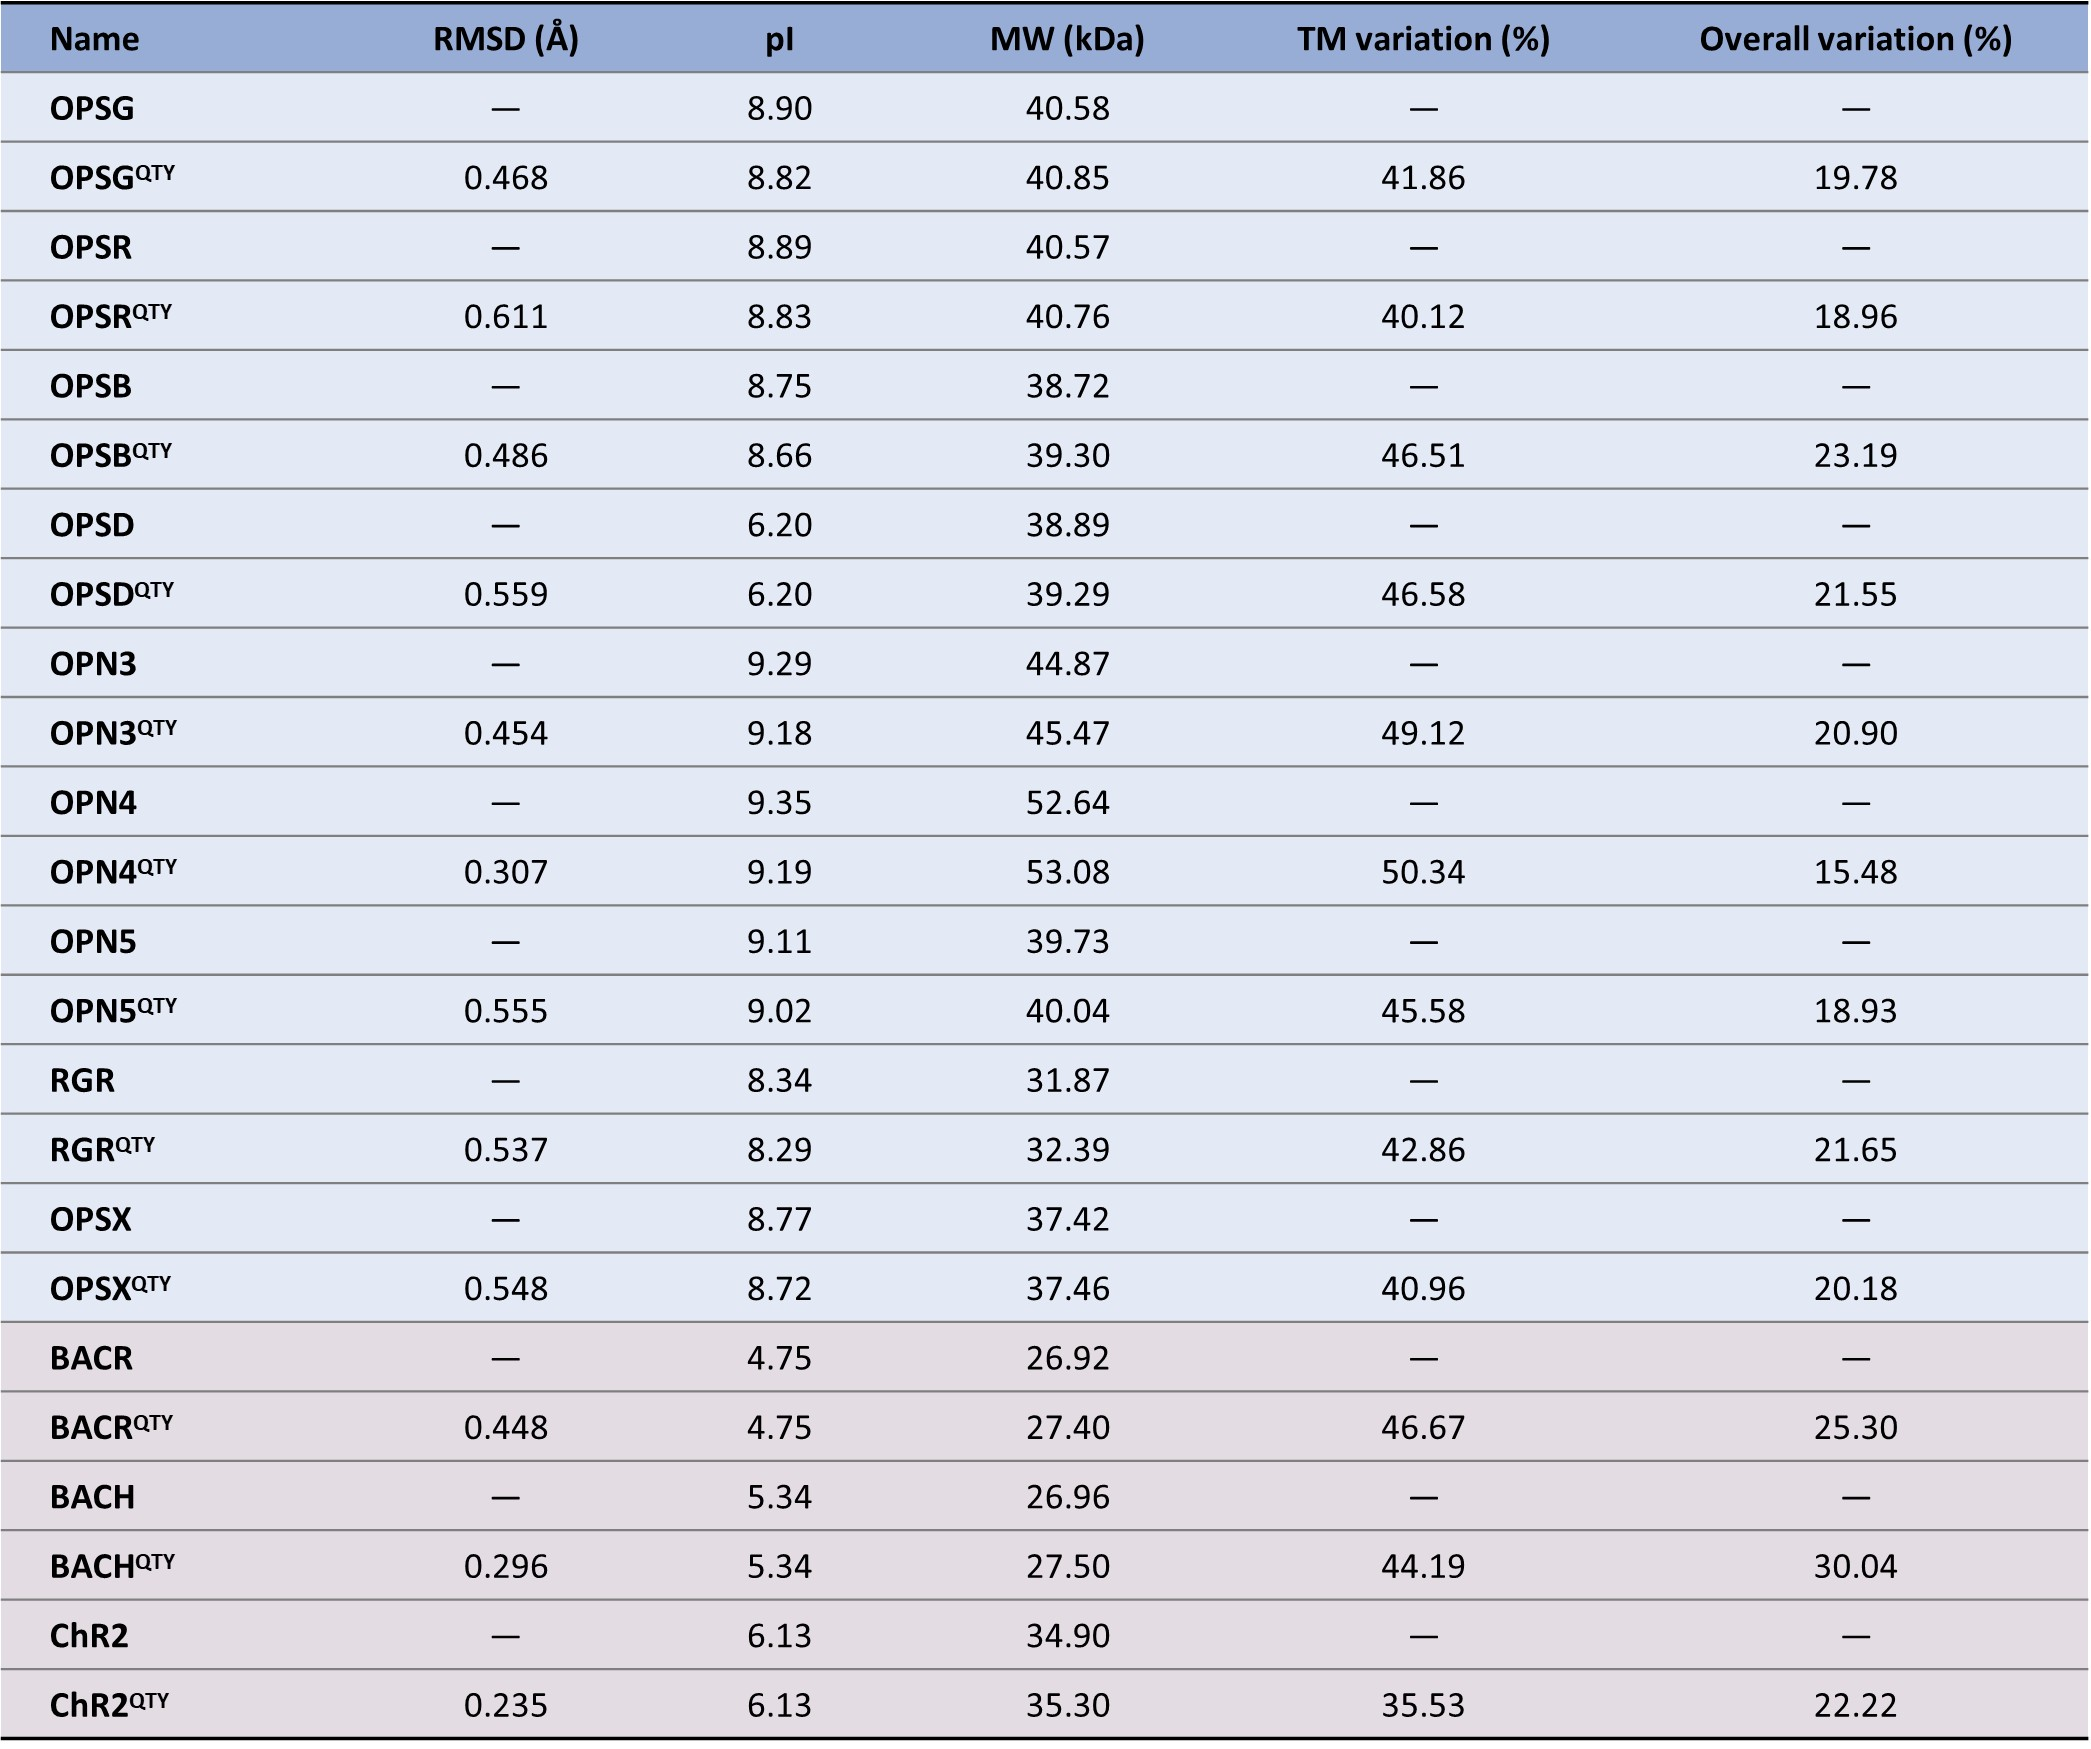
\includegraphics[width=\linewidth]{Figures/characteristics.jpg}
\end{table}


\begin{figure}[h]
	\centering
	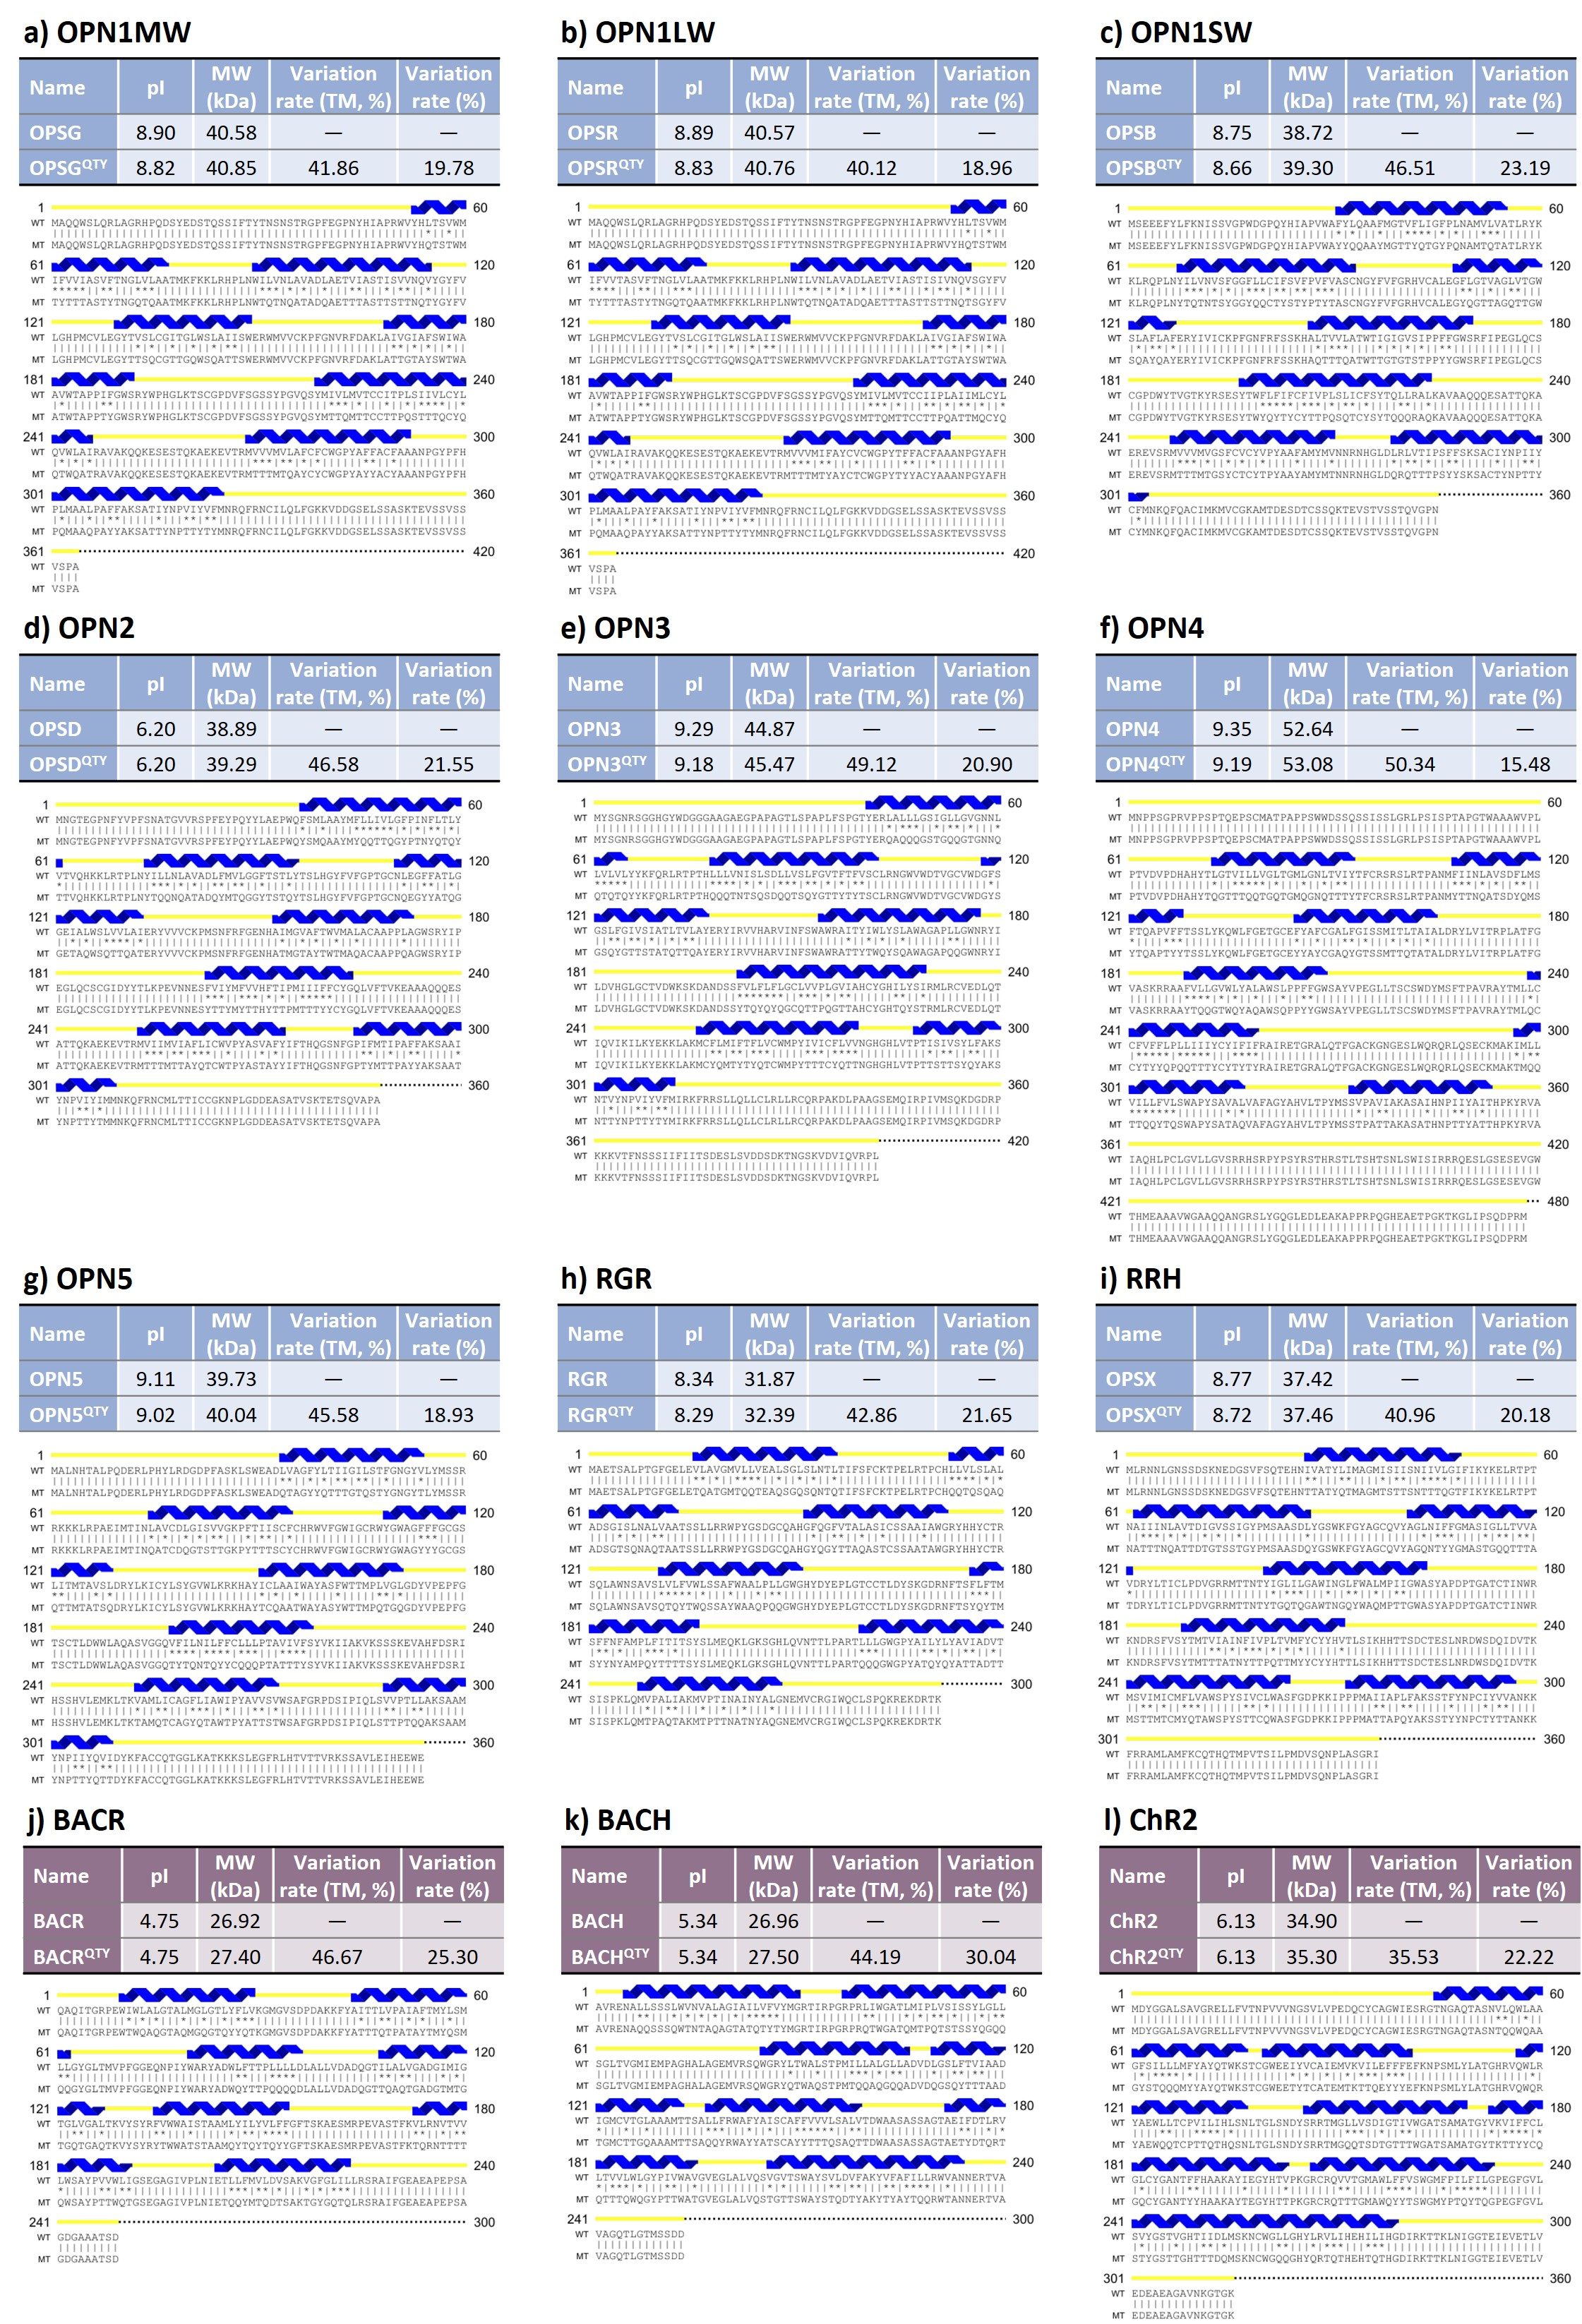
\includegraphics[width=\linewidth]{Figures/sequences.jpg}
	\caption{Protein sequence alignments}
	\label{fig:sequences}
\end{figure}

\begin{figure}[h]
	\centering
	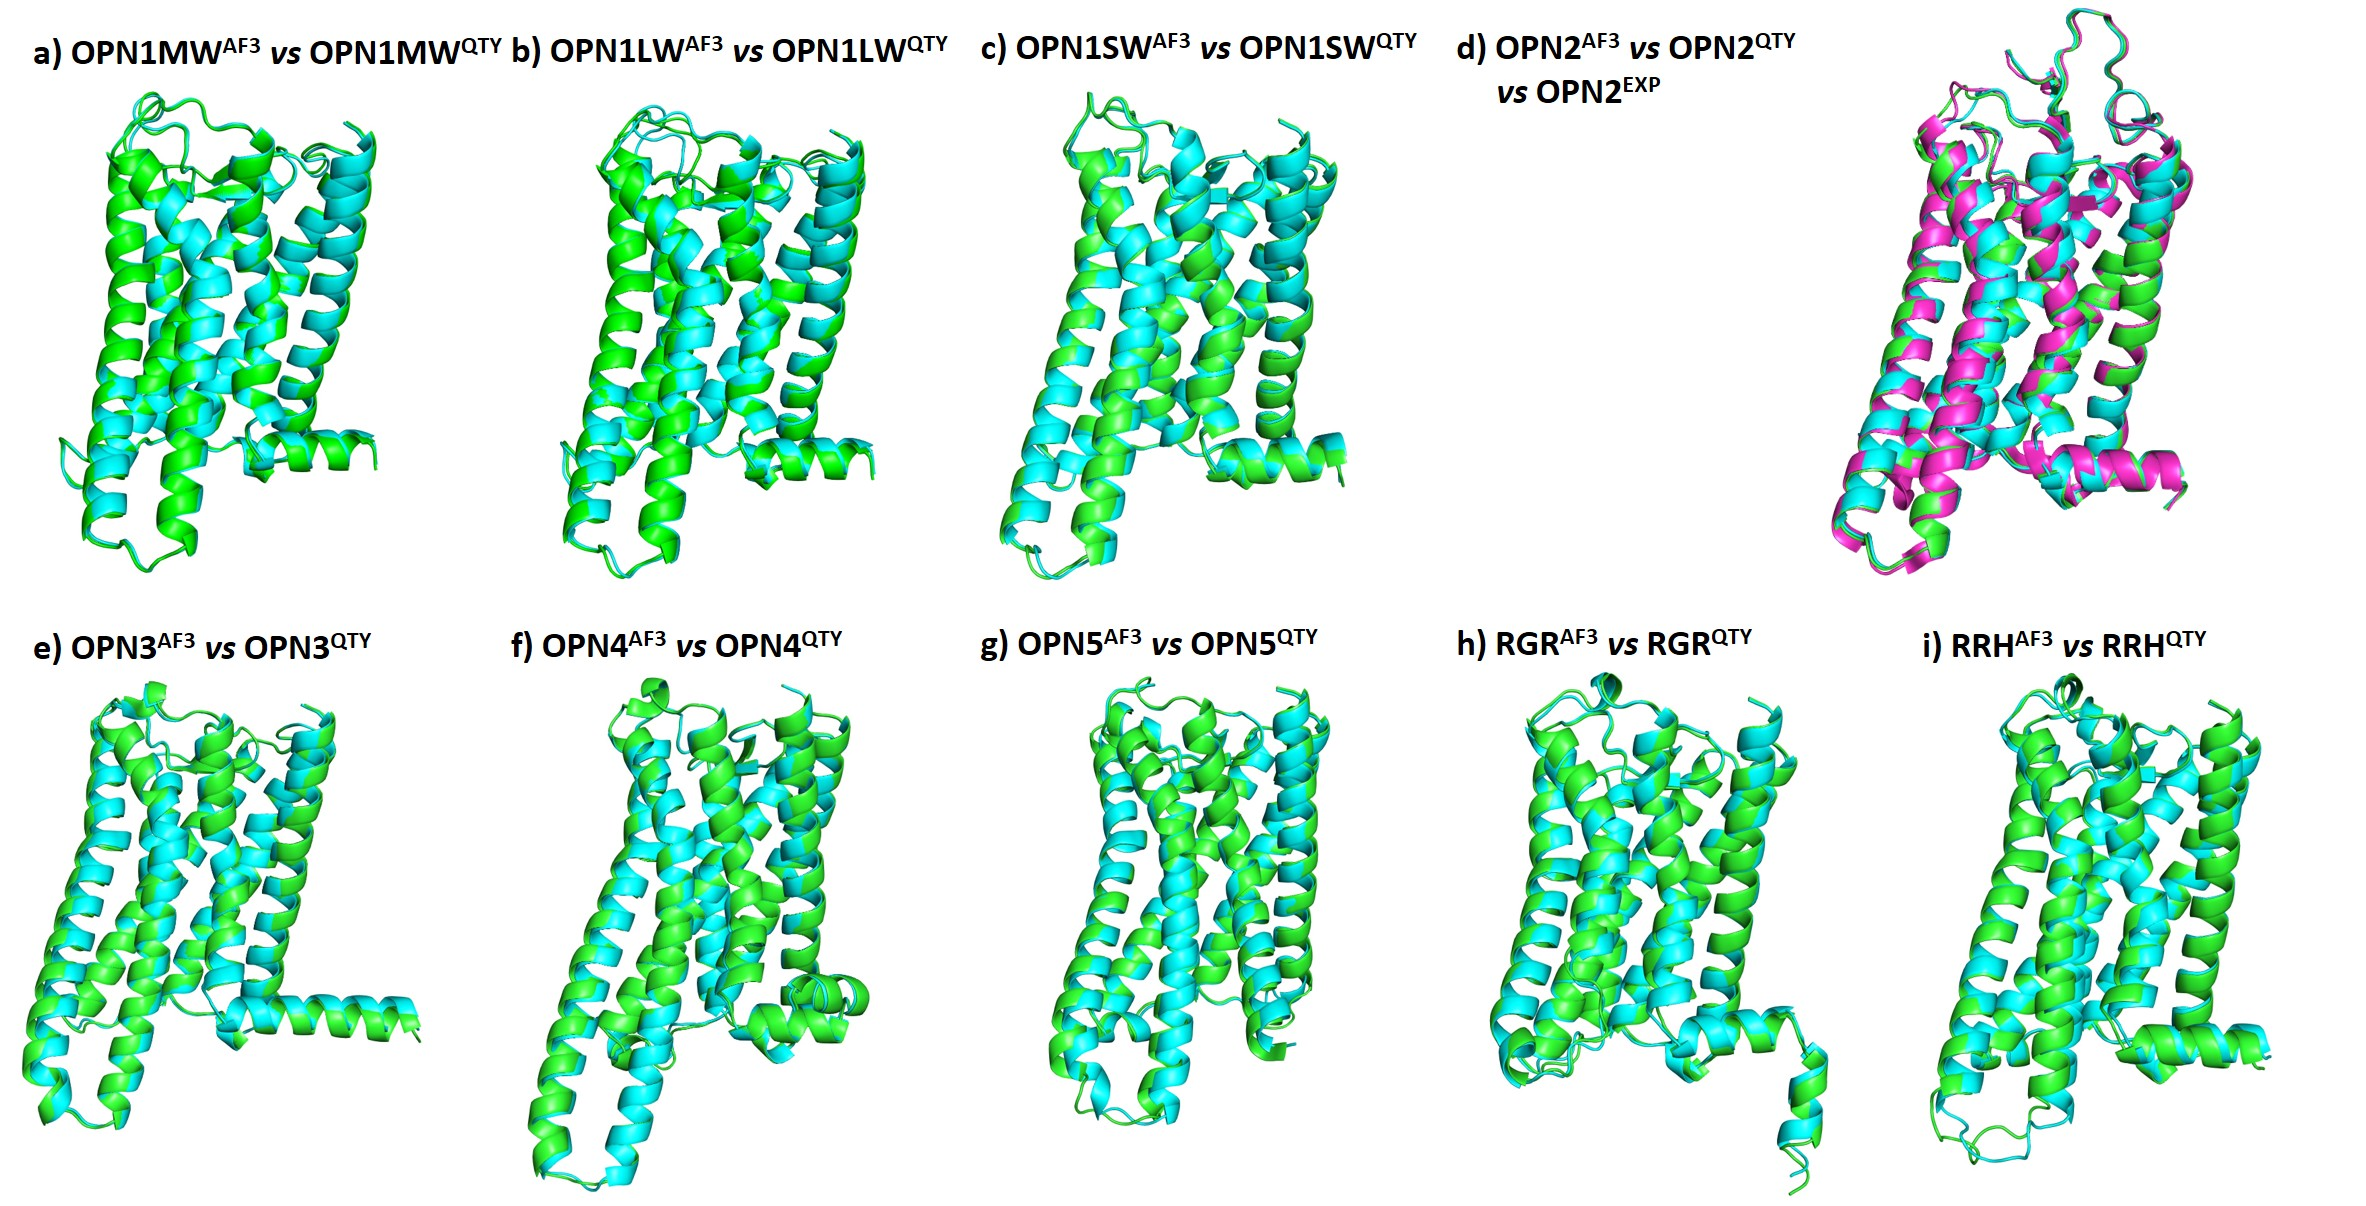
\includegraphics[width=\linewidth]{Figures/superimposition-human.jpg}
	\caption{Superimposition of human retinylidene proteins}
	\label{fig:humansup}
\end{figure}

\begin{figure}[h]
	\centering
	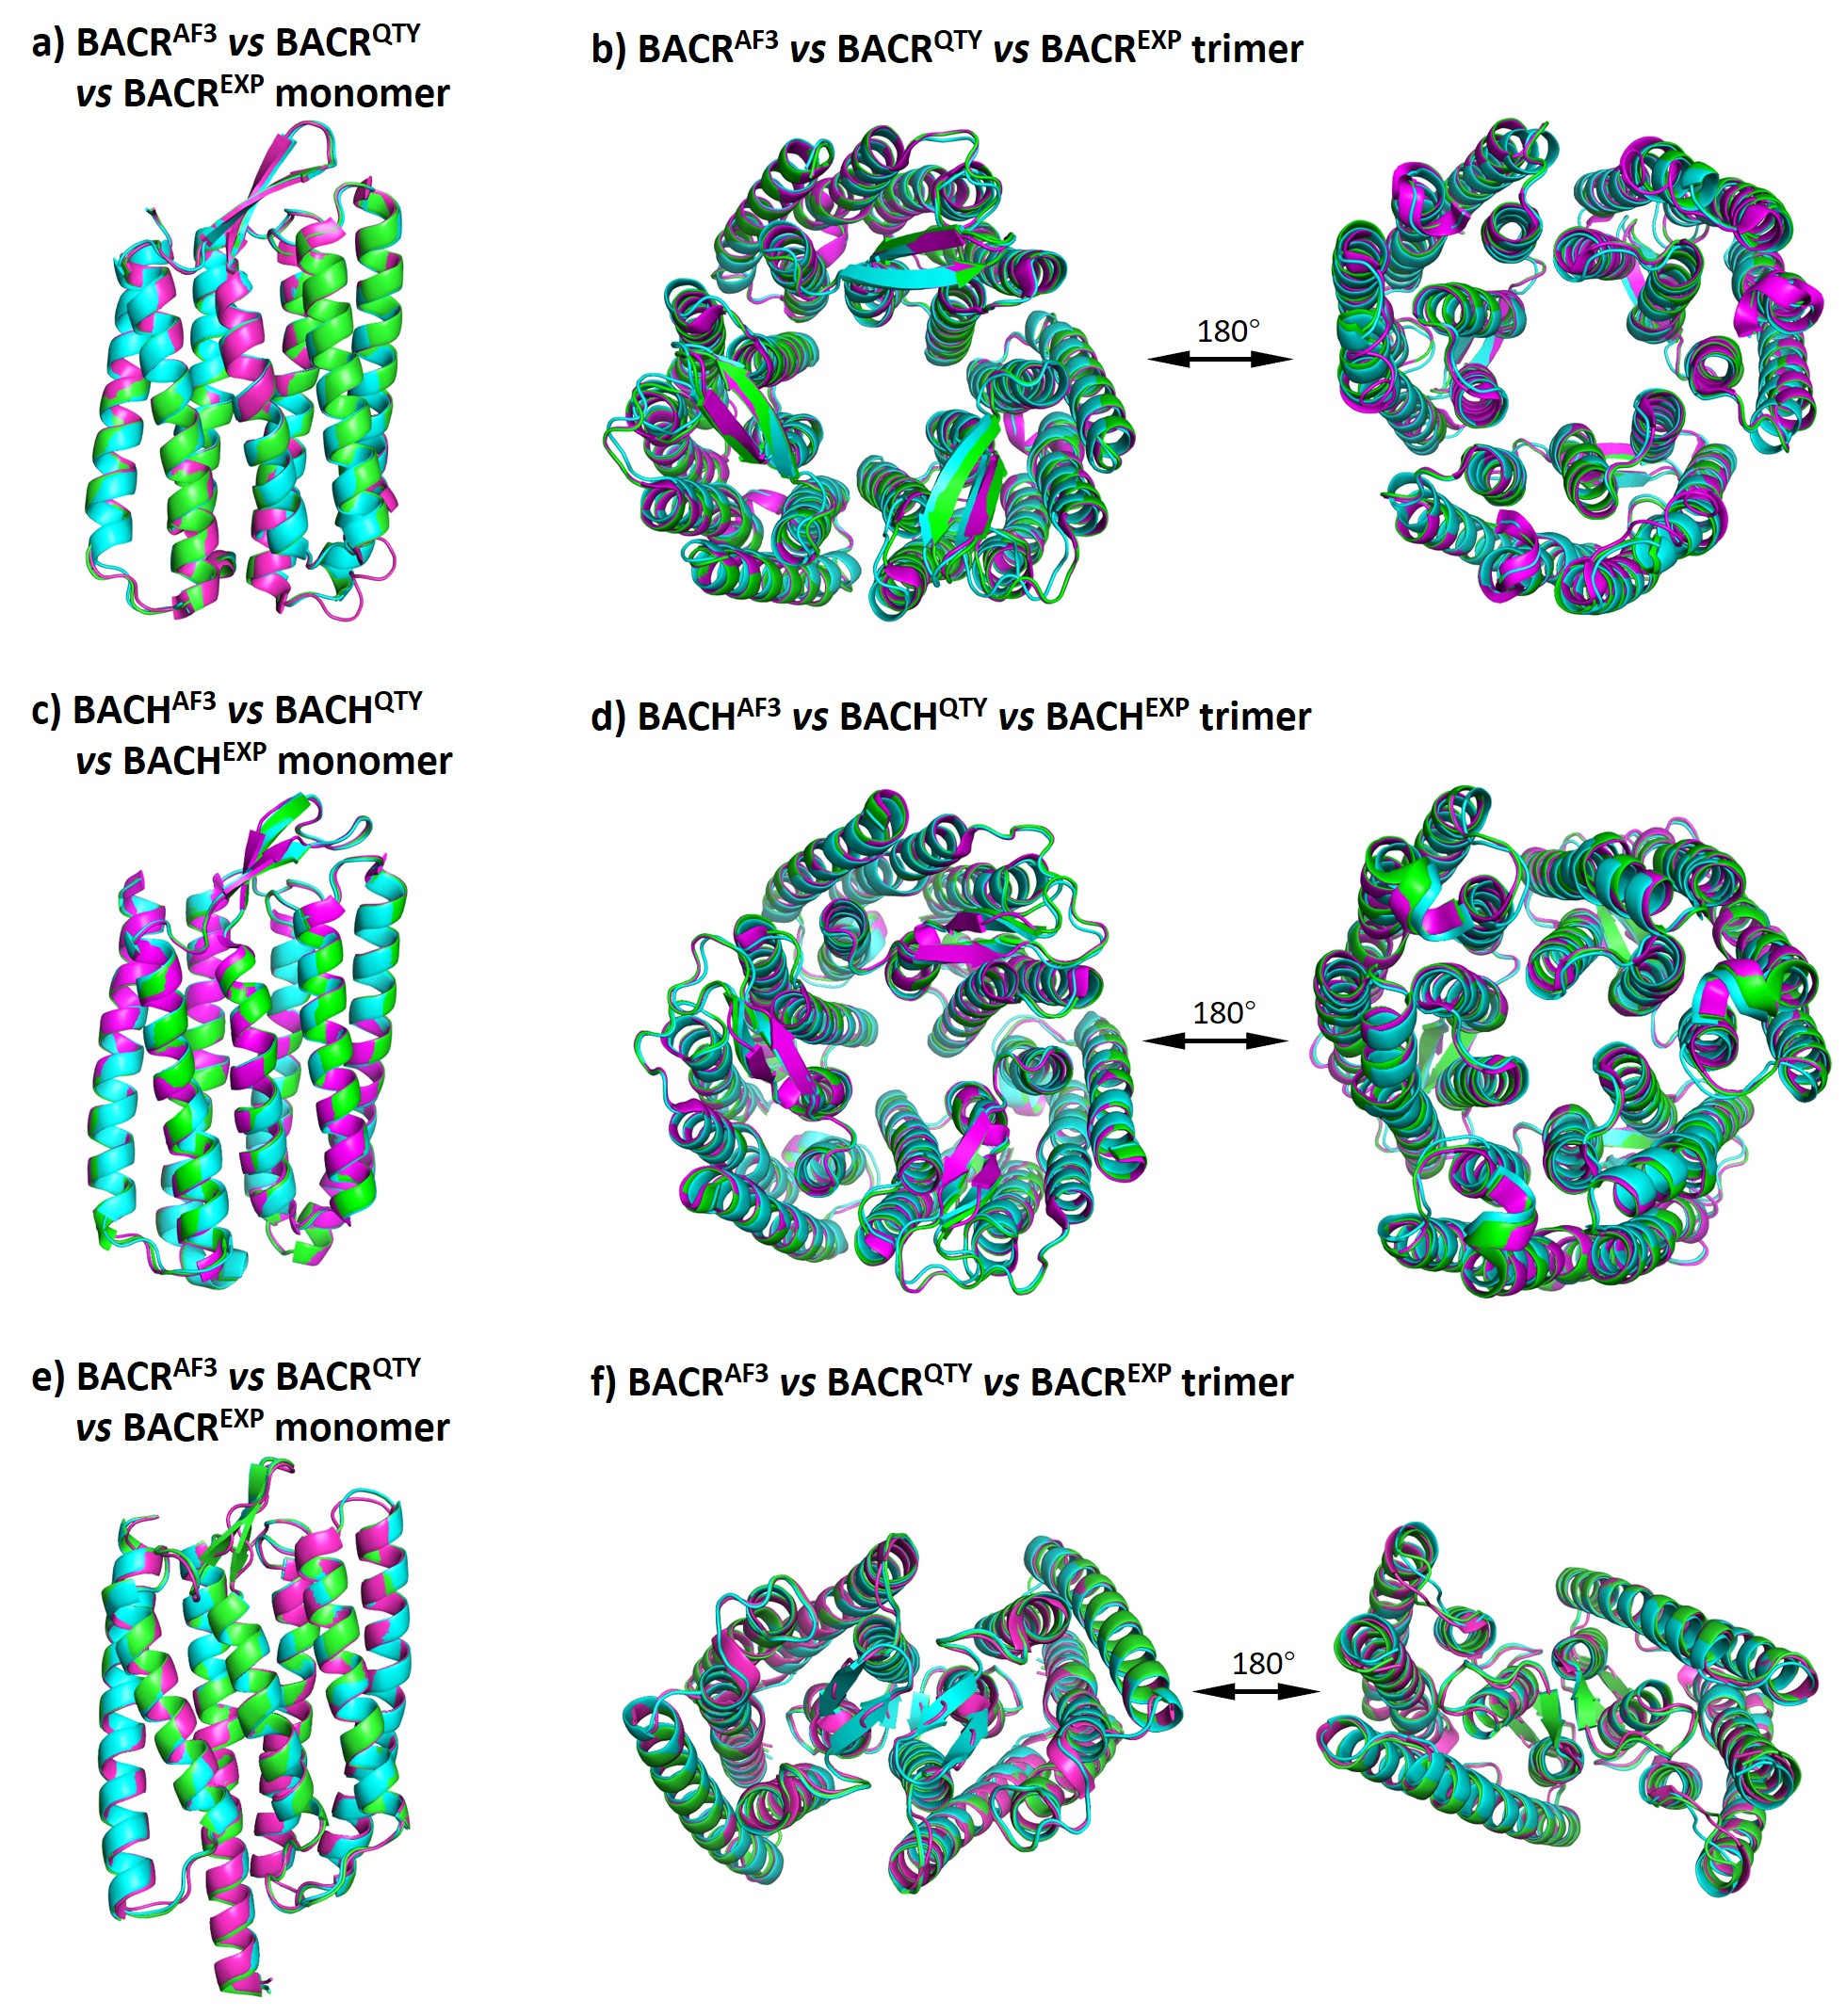
\includegraphics[width=\linewidth]{Figures/superimposition-bacterial.jpg}
	\caption{Superimposition of bacterial retinylidene proteins}
	\label{fig:bacterialsup}
\end{figure}

\begin{figure}[h]
	\centering
	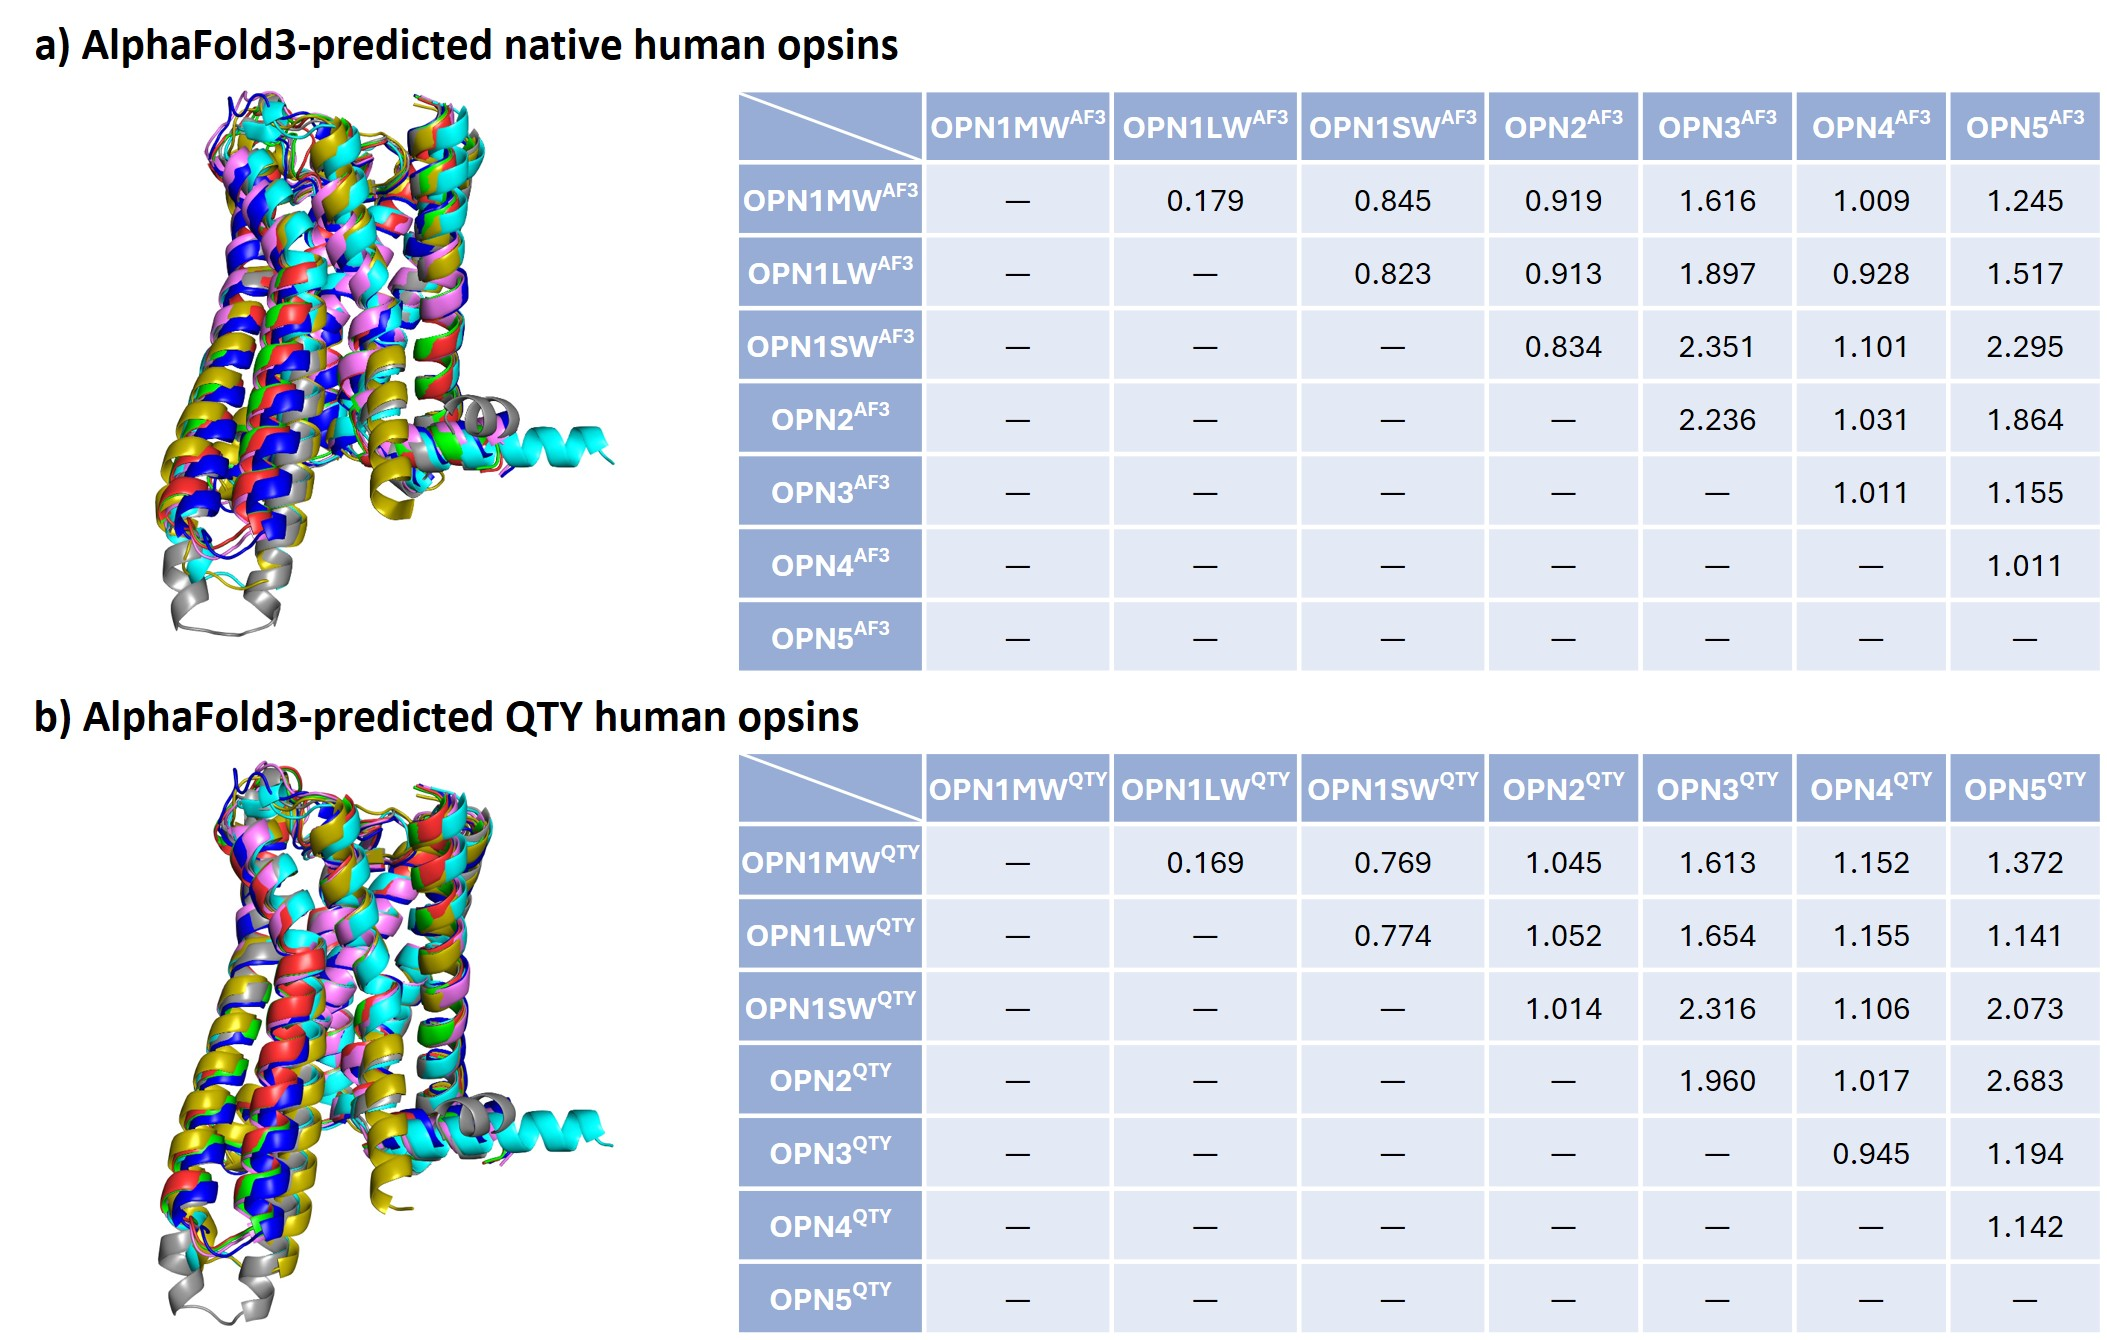
\includegraphics[width=\linewidth]{Figures/pairwise.jpg}
	\caption{Pairwise comparison of human opsins}
	\label{fig:pairwise}
\end{figure}

\begin{figure}[h]
	\centering
	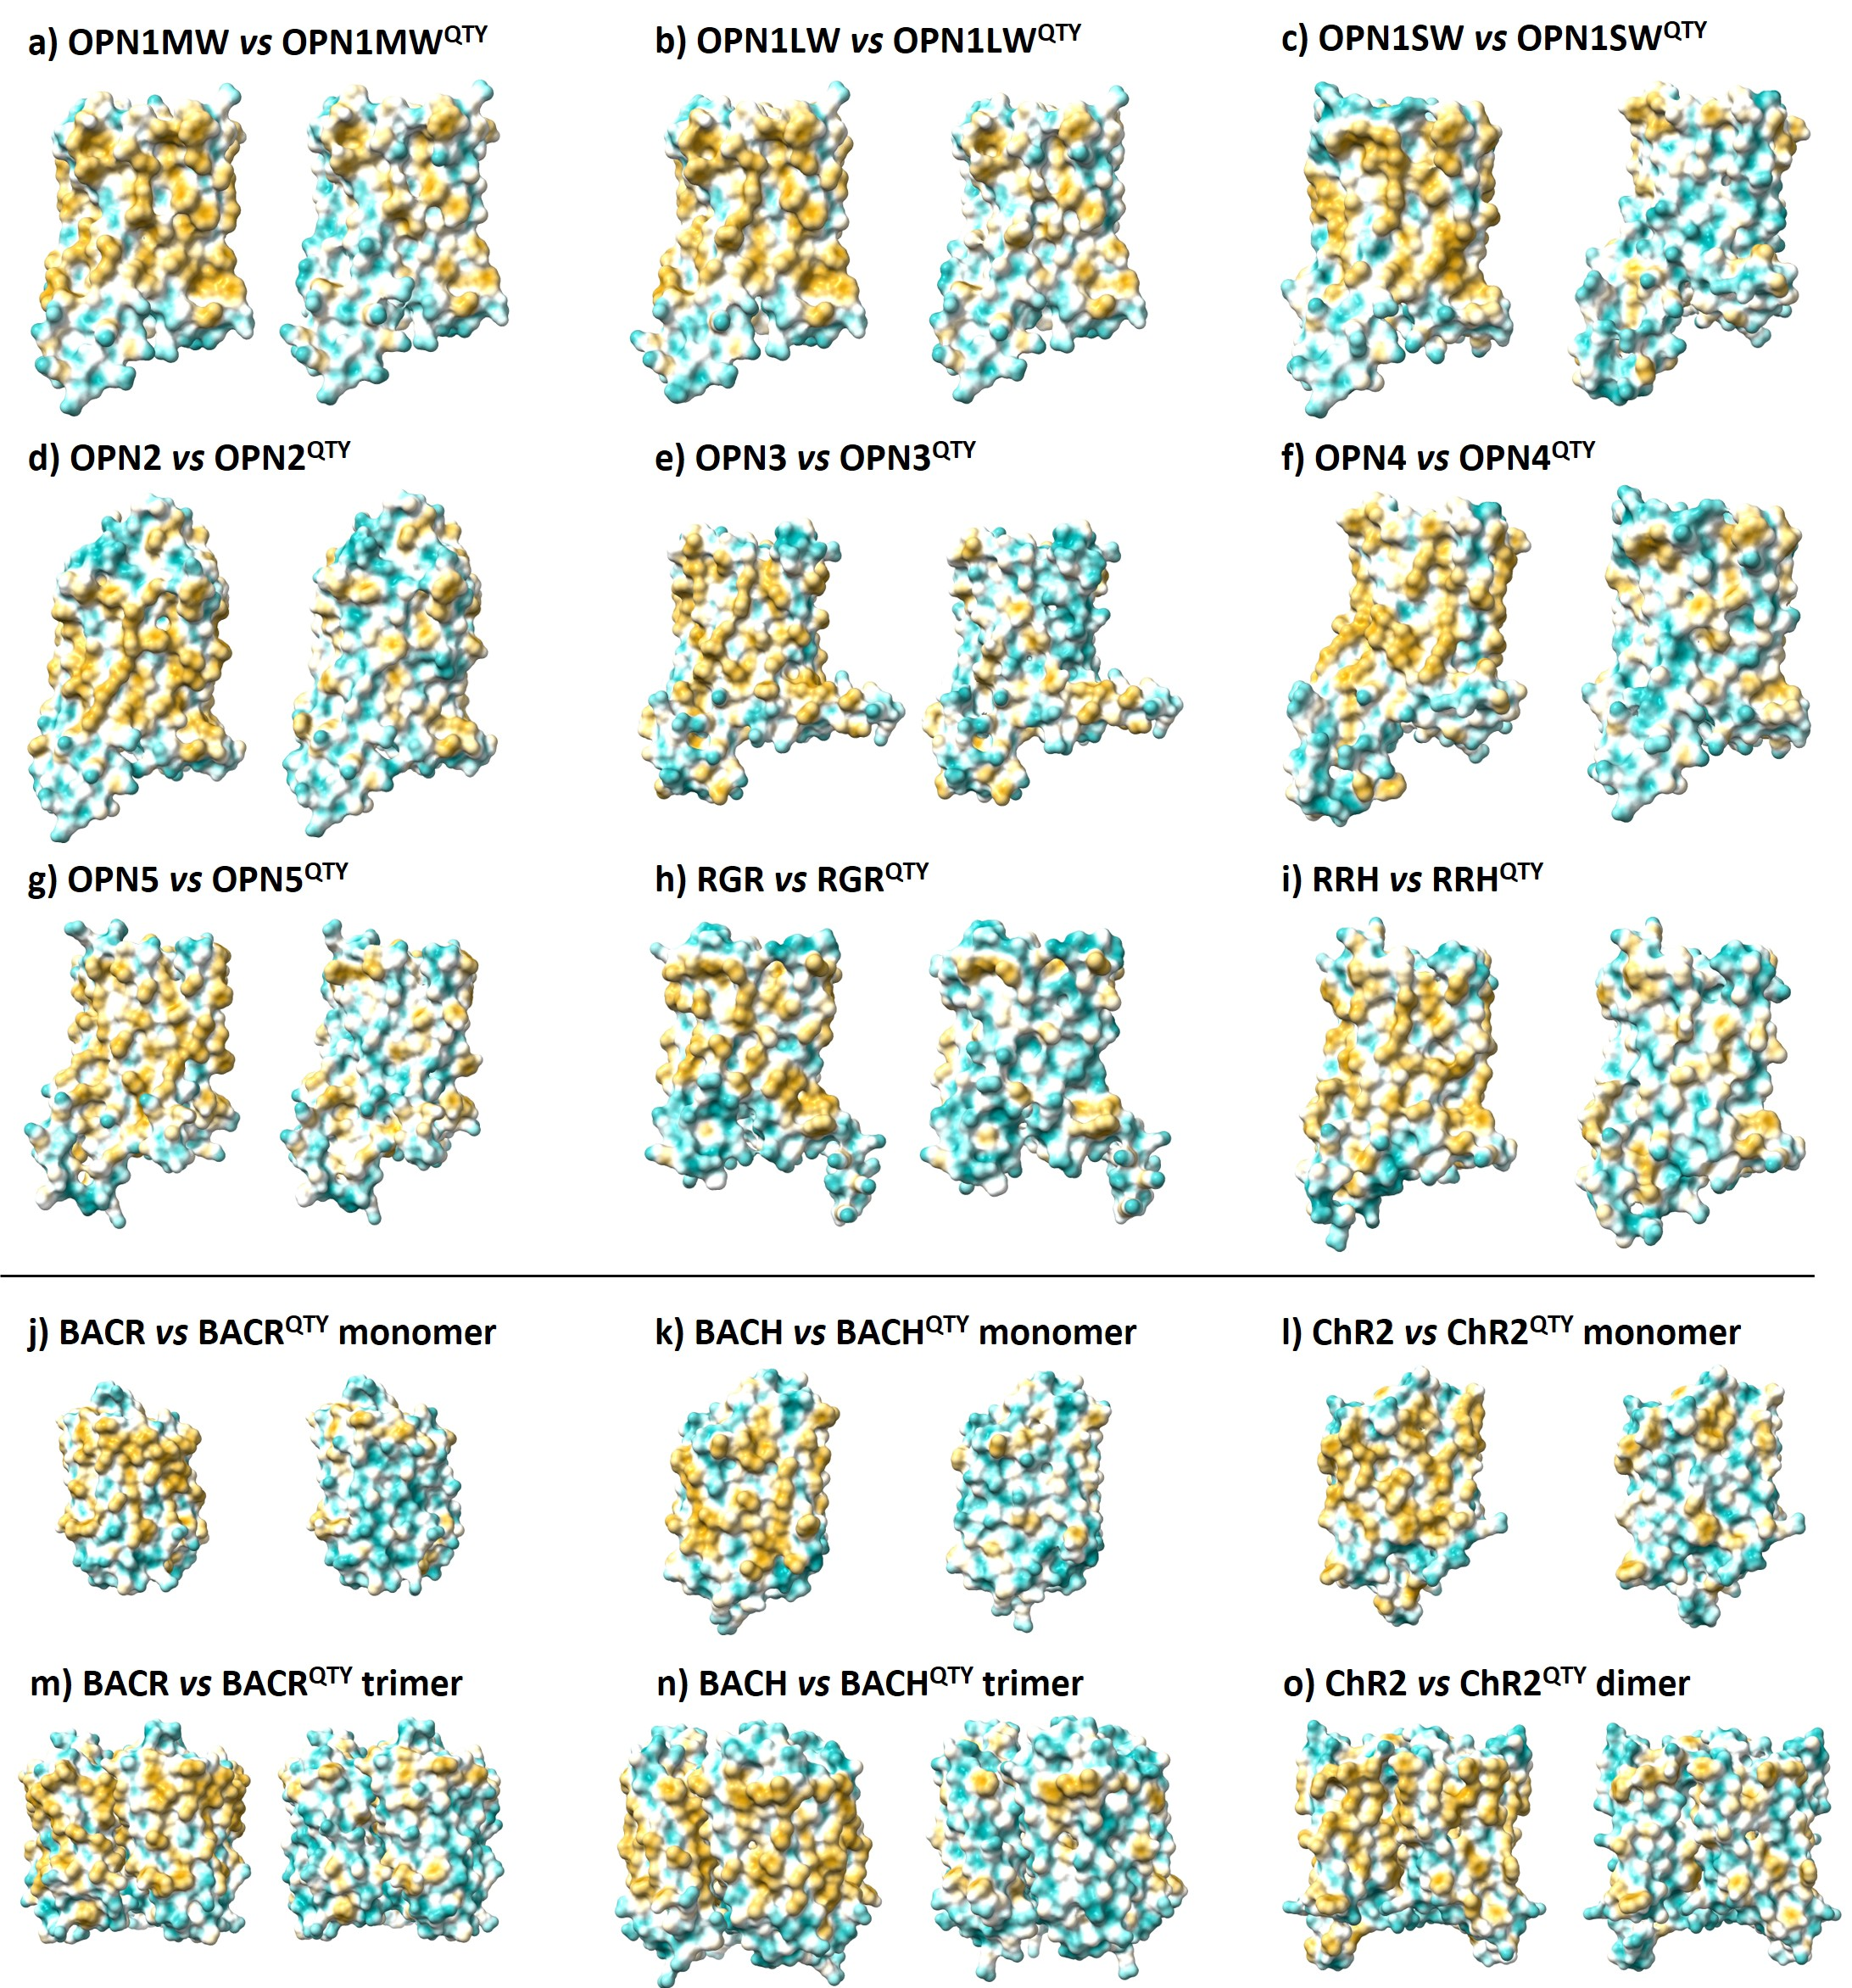
\includegraphics[width=\linewidth]{Figures/hydrophobicity.jpg}
	\caption{Surface hydrophobicity}
	\label{fig:hydrophobicity}
\end{figure}

\end{document}